\documentclass[aspectratio=169]{beamer}

\usepackage{fontspec}
\usepackage{unicode-math}
\usepackage{graphicx}
\usepackage[dvipsnames]{xcolor}
\usepackage[backend=biber,style=numeric,sorting=none]{biblatex}
\usepackage{ragged2e}
\usepackage{setspace}
\usepackage{bookmark}
\usepackage[version=4]{mhchem}
\usepackage[british]{babel}
\usepackage{amsmath}
\usepackage{amssymb}
\usepackage{microtype}
\usepackage{booktabs}
\usepackage{hyperref}
\usepackage{cleveref}

\addbibresource{sainte-chapelle.bib}

\usetheme[numbering=counter, progressbar=frametitle, background=light]{metropolis}

\usecolortheme{dove}
\definecolor{primary}{RGB}{88, 24, 124}
\definecolor{secondary}{RGB}{0, 168, 150}

\setbeamercovered{transparent}
\setbeamercolor{frametitle}{fg=white, bg=primary}
\setbeamercolor{progress bar}{fg=secondary}
\setbeamerfont{frametitle}{size=\large, series=\bfseries}
\setbeamerfont{title}{size=\LARGE, series=\bfseries}
\setbeamercolor{alerted text}{fg=secondary}
\setbeamercolor{block title}{fg=primary}
\setbeamercolor{block body}{bg=white}

\setstretch{1.1}

\setmainfont{Fira Sans}
\setmathfont{TeX Gyre Pagella Math}

\title{The Secret of Sainte-Chapelle}
\subtitle{Thirteenth-Century Nanotechnology in Stained Glass}
\author{Julian Avila \and Bryan Martinez}
\institute{Universidad Distrital Francisco José de Caldas}
\date{\today}

\begin{document}

\begin{frame}
  \titlepage
\end{frame}

\begin{frame}{Outline}
  \setbeamertemplate{section in toc}[sections numbered]
  \tableofcontents
\end{frame}

\section{Historical Context}

\begin{frame}{Introduction and Macroscopic Scale}
  \begin{itemize}
    \item Built between 1243 and 1248 to house the \textbf{Passion relics} of
      King Louis IX.
    \item Contains 660 square metres of stained glass. The glazing took just 
      six years.
    \item Original archives are lost. The physical material is the sole
      historical record.
    \item The recent restoration allowed \textbf{non-destructive} physical
      analysis on 110 original panels.
  \end{itemize}
\end{frame}

\begin{frame}{Architectural Topology}
  \begin{figure}[h!]
    \centering
    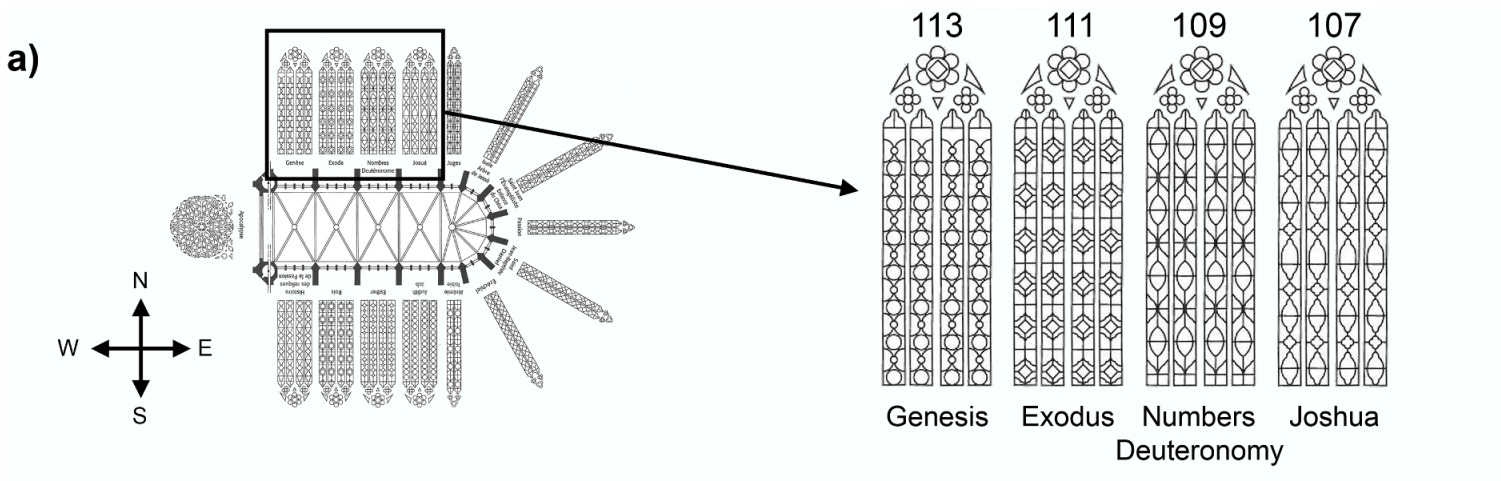
\includegraphics[height=0.6\textheight]{images/arquitectura_capilla.png}
    \caption{The spatial configuration of the four windows restored between
    2011 and 2014 within the Sainte-Chapelle.}
  \end{figure}
\end{frame}

\begin{frame}{Studied Panels}
  \begin{figure}[h!]
    \centering
    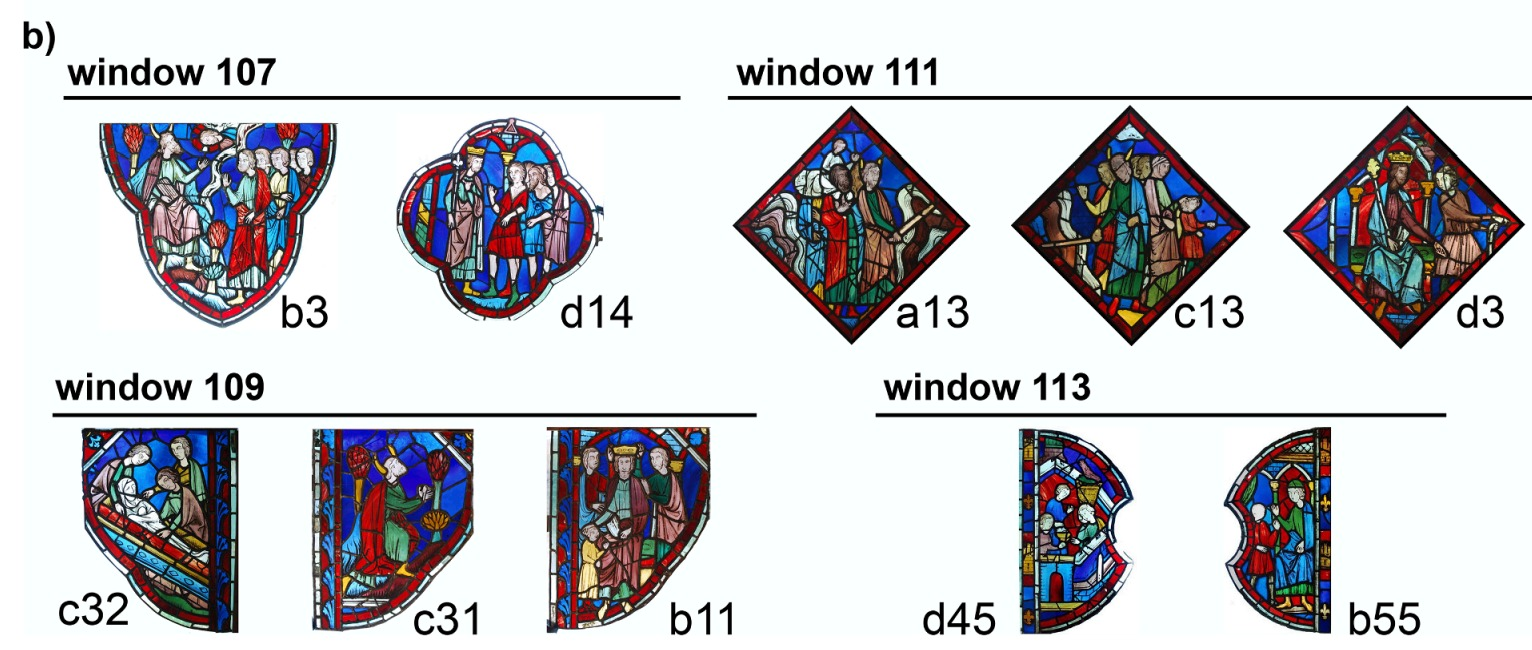
\includegraphics[height=0.6\textheight]{./images/vidrios_capilla.png}
    \caption{A selection of the historical glass panels analyzed.}
  \end{figure}
\end{frame}

\section{Material Composition}

\begin{frame}{The Glass Matrix and Network Modification}
  \begin{itemize}
    \item The matrix is an amorphous solid. \textbf{Silica} acts as the primary
      network former.
    \item Plant ash provides potassium oxide. This acts as the \textbf{network
      modifier}.
    \item The glass has the highest silica fraction recorded in medieval Europe.
    \item This yields a rigid network. It requires high melting temperatures
      but ensures \textbf{exceptional durability}.
  \end{itemize}
\end{frame}

\begin{frame}{Compositional Topology}
  \begin{figure}
    \centering
    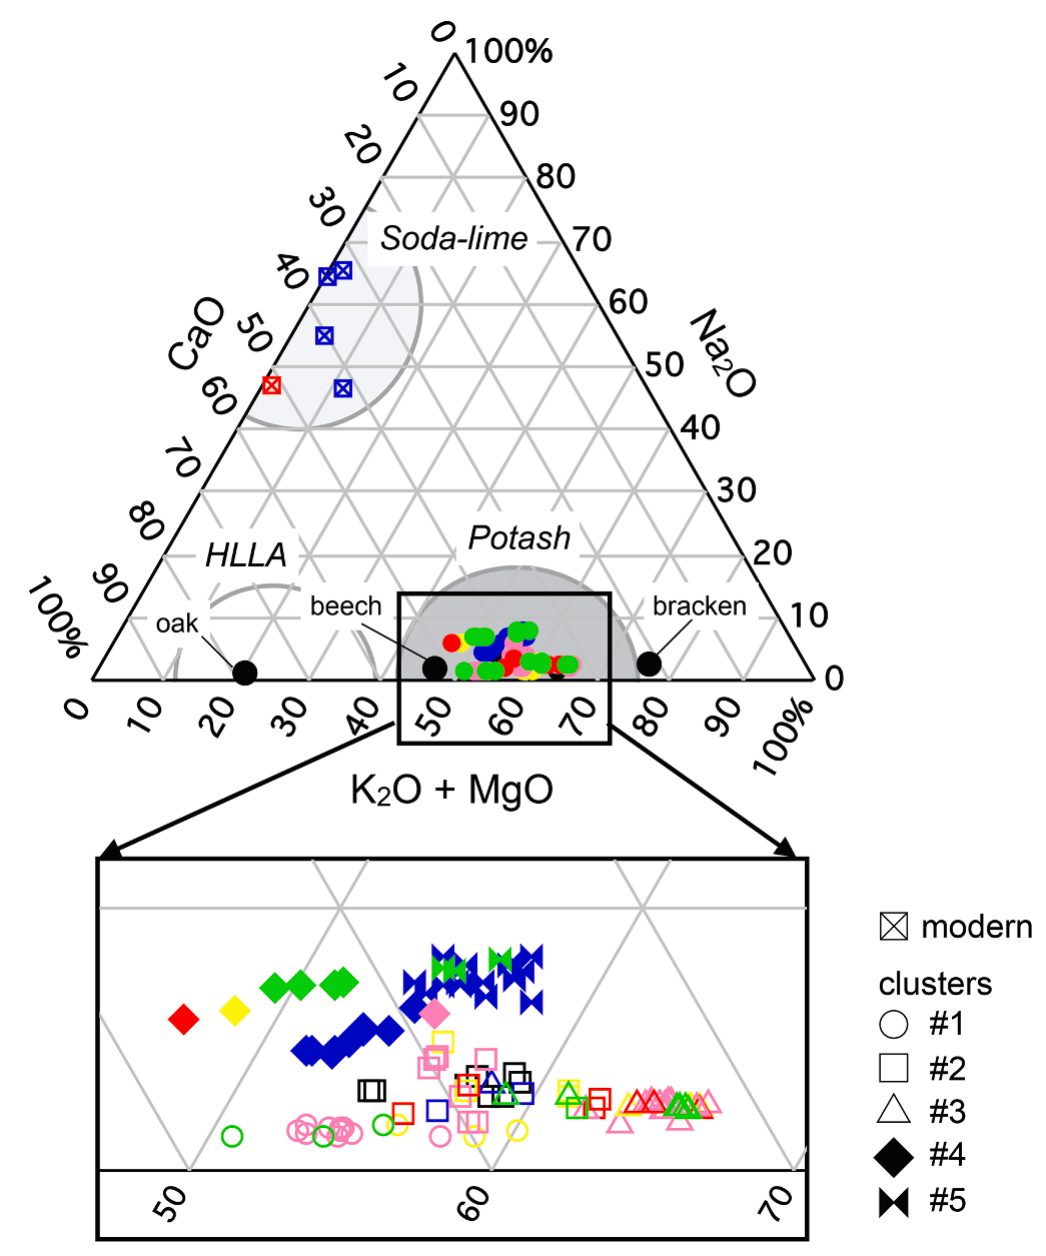
\includegraphics[height=0.7\textheight]{./images/ternary-graph.png}
    \caption{Ternary phase diagram illustrating the mass fractions of the
    primary glass constituents.}
  \end{figure}
\end{frame}

\section{Optical Properties and Chromophores}

\begin{frame}{Chromophores and Redox Equilibrium}
  \begin{itemize}
    \item Macroscopic colour stems from transition metal ions. These act as
      localised \textbf{chromophores}.
    \item Colourless, yellow, and purple hues depend strictly on thermodynamic
      equilibrium.
    \item This relies on a delicate \textbf{redox balance} between iron
      (\ce{Fe^{2+}}, \ce{Fe^{3+}}) and manganese (\ce{Mn^{2+}}, \ce{Mn^{3+}})
      states.
  \end{itemize}
\end{frame}

\begin{frame}{Optical Absorption in the Visible Spectrum}
  \begin{figure}
    \centering
    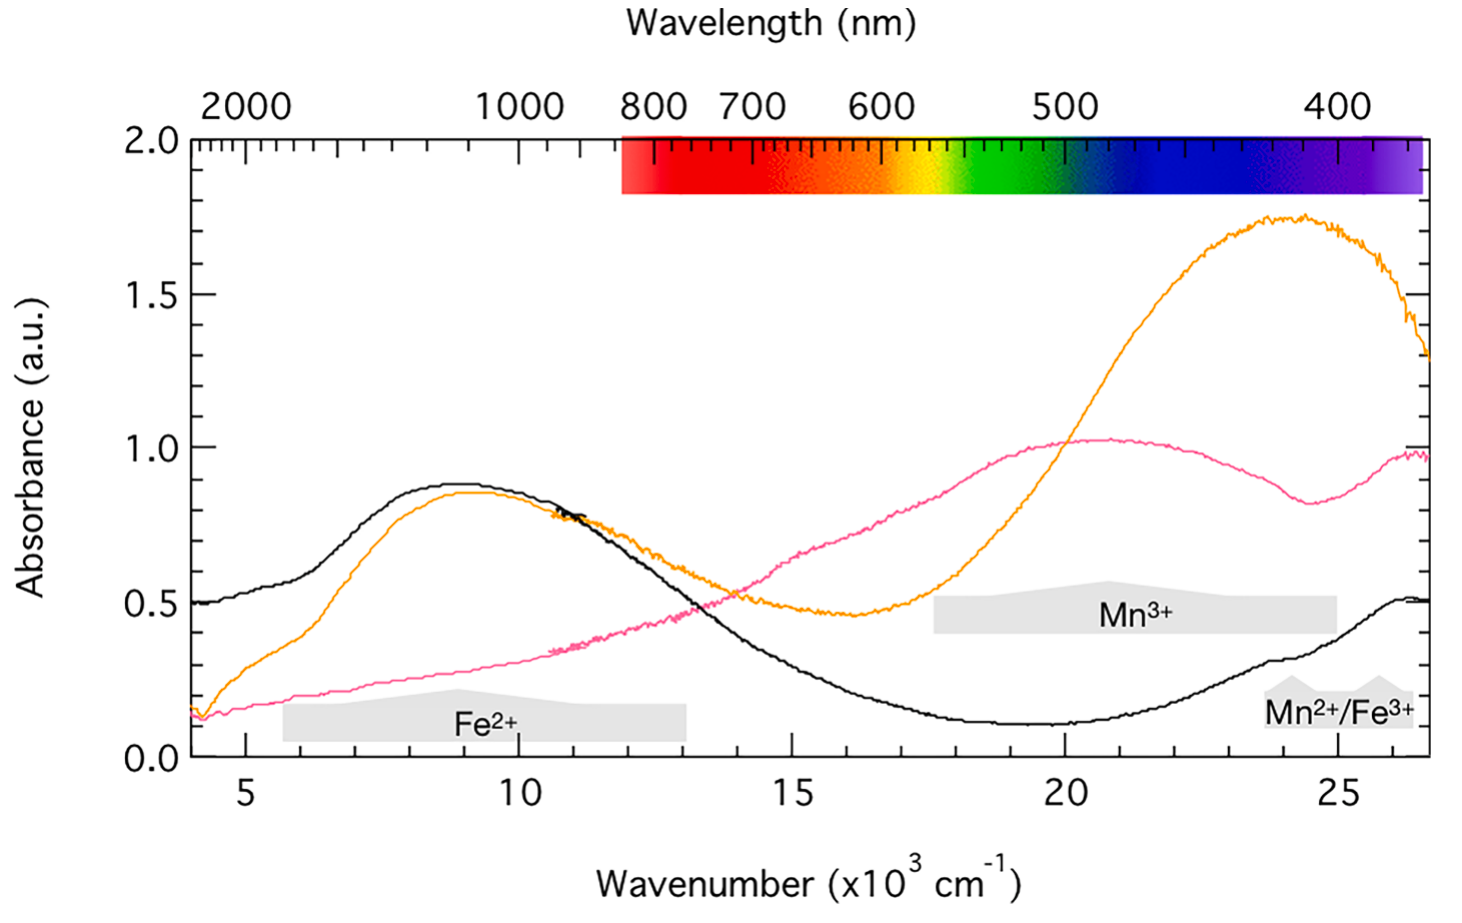
\includegraphics[height=0.7\textheight]{./images/absorption-cpy.png}
    \caption{Optical absorption spectra for colourless, purple, and yellow
    glasses.}
  \end{figure}
\end{frame}

\begin{frame}{Transition Metal Concentrations}
  \begin{figure}
    \centering
    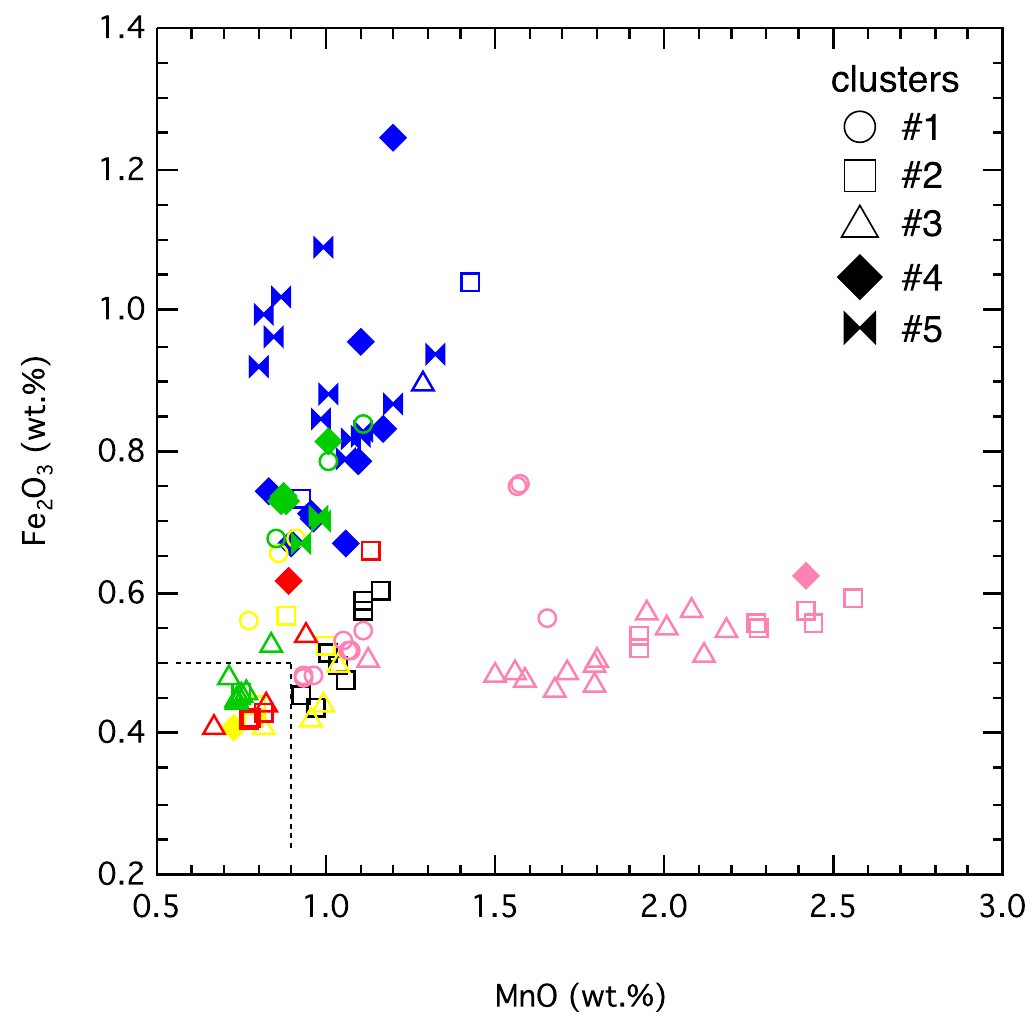
\includegraphics[height=0.7\textheight]{./images/fe-vs-mn.png}
    \caption{Concentration of iron versus manganese expressed as total
    oxides.}
  \end{figure}
\end{frame}

\begin{frame}{The Blue and Green Chromophores}
  \begin{itemize}
    \item Blue transmission is dictated by \ce{Co^{2+}} ions from imported
      German saffre.
    \item Green hue is a \textbf{superposition} of absorption states.
    \item High \ce{Cu^{2+}} oxidises iron to \ce{Fe^{3+}}. The copper and iron
      combine to define the green frequency.
  \end{itemize}
\end{frame}

\begin{frame}{Optical Absorption of Blue Glass}
  \begin{figure}
    \centering
    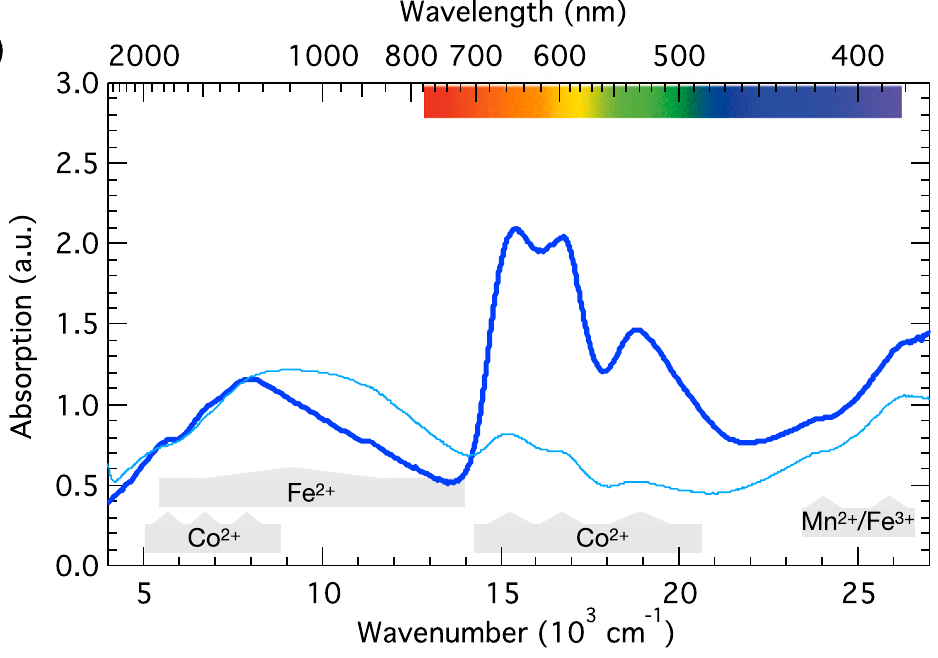
\includegraphics[height=0.7\textheight]{./images/absorption-blue.png}
    \caption{Optical absorption spectra contrasting light and dark blue
    glass matrices.}
  \end{figure}
\end{frame}

\begin{frame}{Trace Element Correlation in Blue Glass}
  \begin{figure}
    \centering
    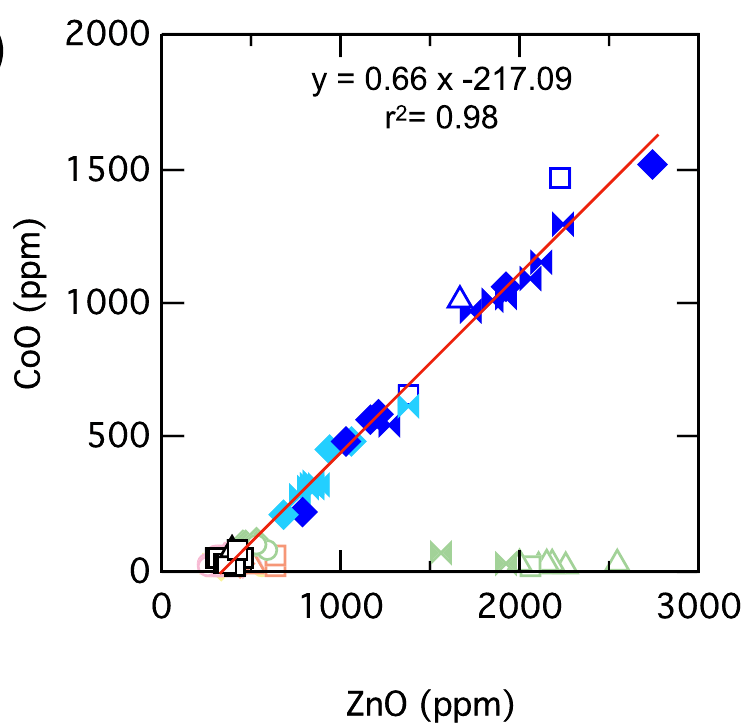
\includegraphics[height=0.7\textheight]{./images/co-vs-zn.png}
    \caption{Concentration of cobalt relative to the amount of zinc oxide.}
  \end{figure}
\end{frame}

\begin{frame}{Optical Absorption of Green and Red Glasses}
  \begin{figure}
    \centering
    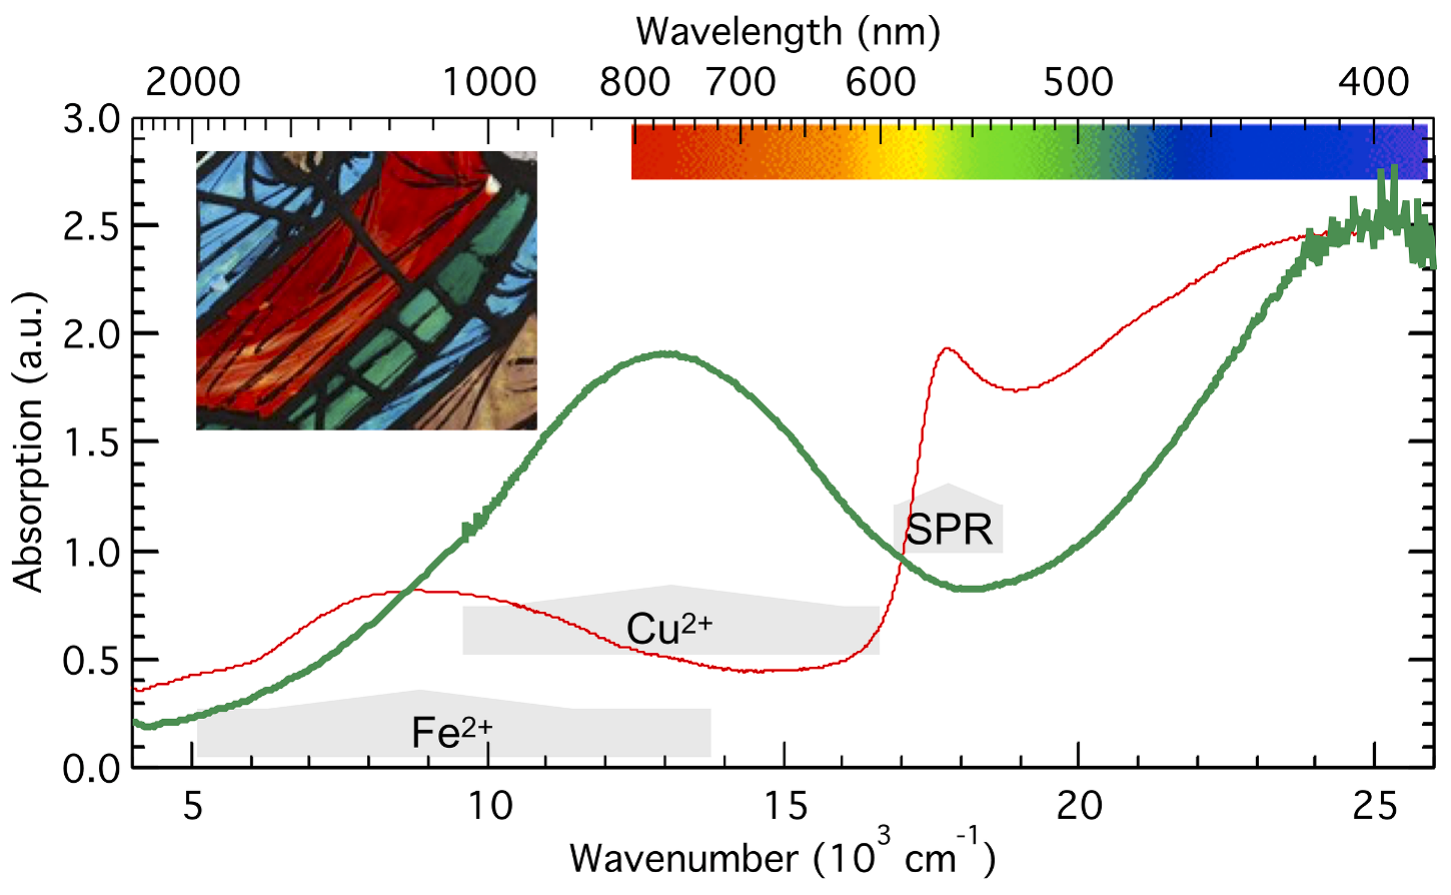
\includegraphics[height=0.7\textheight]{./images/absorption-green.png}
    \caption{Optical absorption spectra for green and red glasses.}
  \end{figure}
\end{frame}

\begin{frame}{Trace Element Correlation for Copper Inclusions}
  \begin{figure}
    \centering
    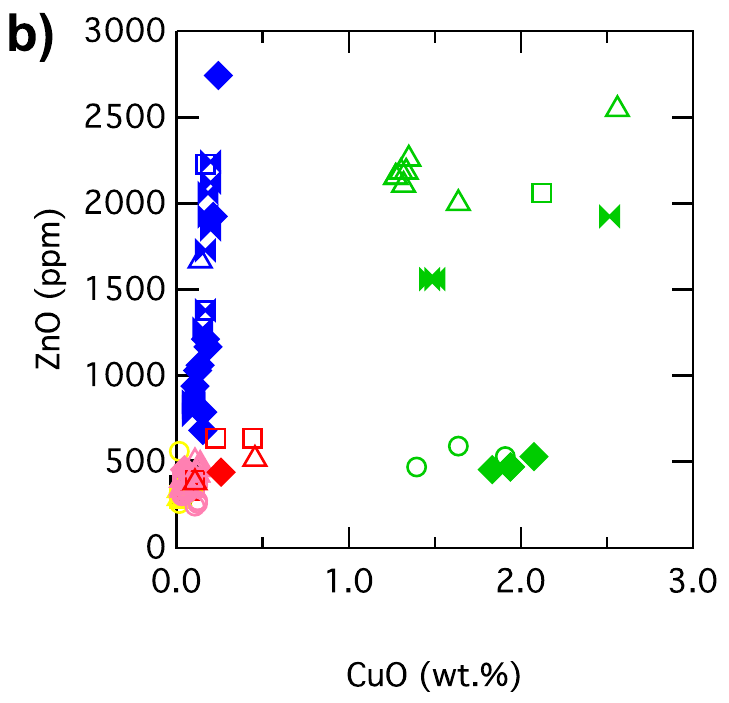
\includegraphics[height=0.7\textheight]{./images/zno-vs-cuo.png}
    \caption{Amount of zinc oxide plotted against copper oxide.}
  \end{figure}
\end{frame}

\section{Nanotechnology and Analytical Methods}

\begin{frame}{Nanoscale Topology and Surface Plasmon Resonance}
  \begin{itemize}
    \item Red colour is not from dissolved ions. It originates from
      \textbf{metallic copper nanoparticles}.
    \item The electromagnetic field couples to the electron plasma, driving
      \textbf{surface plasmon resonance}.
    \item To maintain optical translucency, the glass is \textbf{striated}. It
      alternates red and colourless microscopic layers.
  \end{itemize}
\end{frame}

\begin{frame}{Nanoparticle Kinematics and Sizing}
  \begin{itemize}
    \item The mean radius $R$ of the copper inclusions is derived from the
      \textbf{full width at half maximum} ($\Gamma$) of the SPR band.
    \item Applying the Drude free-electron model to Mie scattering theory
      yields the boundary condition:
      \[ R = \frac{v_F}{\Gamma - \Gamma_0} \]
    \item Here, $v_F$ is the \textbf{Fermi velocity} of the electron plasma in
      metallic copper.
    \item This calculation isolates the quantum confinement, determining the
      nanoparticles are approximately \textbf{15 nm} in size.
  \end{itemize}
\end{frame}

\begin{frame}{Non-Destructive Ion Beam Analysis}
  \begin{itemize}
    \item Elemental characterisation used the AGLAE accelerator. This preserved
      the artefacts' topology.
    \item A 3 MeV proton beam induced inner-shell \textbf{ionisation} and
      nuclear \textbf{resonant transitions}.
    \item X-ray and gamma-ray emissions were recorded simultaneously to map
      elemental mass fractions.
  \end{itemize}
\end{frame}

\begin{frame}{Statistical Resolution of the Matrix}
  \begin{itemize}
    \item The proton beam traverses multiple layers. This yields an integrated,
      obscured signal.
    \item \textbf{Hierarchical cluster analysis} was applied to the emission
      data to isolate the base composition.
    \item Using Euclidean distances, this resolved \textbf{five distinct}
      compositional boundaries.
  \end{itemize}
\end{frame}

\section{Conclusion}

\begin{frame}{Physical and Historical Conclusions}
  \begin{itemize}
    \item The analysis successfully identified five clusters of \textbf{potash
      glass}.
    \item The glass matrix and chromophores show a uniform spatial distribution
      across all structural windows.
    \item This macroscopic uniformity proves the four windows were glazed
      \textbf{simultaneously}.
    \item It implies a single master atelier using a \textbf{unified material
      supply}.
  \end{itemize}
\end{frame}

\begin{frame}[allowframebreaks]{References}
  \printbibliography
  \nocite{*}
\end{frame}

\begin{frame}[plain]
  \centering
  \vspace{1cm}
  {\Huge Thank you.}\\[1cm]
  {\large Questions or comments?}
\end{frame}

\end{document}
